\chapter{Introduction}
\setcounter{page}{1}

\section{Background and Motivation}

In the 21st century, Climate change is the biggest challenge faced by humanity. It poses a substantial danger to the survival of the inhabitants of our planet.
Human activities such as deforestation and burning of fossil fuels have led to a rise in global temperatures.
Becuase of this rise, there has been a rise in sea levels, extreme weather events, and loss of biodiversity.
There is an urgent need to reduce greenhouse gas emissions and transition to a sustainable, low-carbon future.

Maritime is essential to the global economy, transporting 90\% of the world's goods by volume.
It is also a major source of greenhouse gas emissions, with the International Maritime Organization (IMO)
estimating that maritime shipping accounts for 3\% of global carbon dioxide emissions.
While 3\% may seem small, it is important to note that this is a rapidly growing sector.
Without action, maritime shipping contribution to carbon emissions can increase upto 10-13\% in the next few decades..
Due to this fact, there is a growing global effort to reduce emissions from this sector. \autocite{king_anthony_2022}.

In accordance with sustainable Development Goal 13, in 2018, the inital stratergy was adopted by IMO's Environmental Protection Committee (MEPC),
during its 72nd session at IMO Headquarters in London, United Kingdom. Accorging to this stratergy,
the IMO will work towards reducing the total annual greenhouse gas emissions from international shipping by at least 50\% by 2050 compared to 2008 \autocite{imo-2018}.
In 76th ssssion MEPC in 2021, serval mandatory measures were adopted to reduce greenhouse gas emissions from international shipping,
which will help in achieving the goal of reducing emissions by 50\% by 2050 \autocite{imo-2021}. One of the important measures is the carbon intensity indicator (CII).

\begin{figure}[ht]
    \centering
    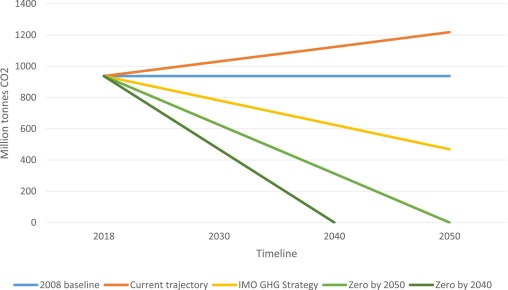
\includegraphics[width=0.7\textwidth]{images/emission_trajactory.jpg}
    \caption{Emission trajectories for different levels of ambition for emission reduction targets}
    \label{emissionTrajectory}
\end{figure}


Maritime shipping is a complex and highly volatile system, generating very large data sets.
Big data analytics can be used to understand the complex system and make informed decisions.
It can facilitate operations such as monitoring of emission and predictive analysis of vessel performance.
This can help in reducing emissions and improving the efficiency of the maritime sector \autocite{ZAMAN2017537}.


\section{Big Data Analysis}

Big data analytics is where advanced analytic techniques operate on big data sets. Hence, big data
analytics is really about two things — \textit{big data} and \textit{analytics}.



\subsection{Big Data}

As the name suggests, big data is a large amount of data. There are other important attributes of big data. These are:  data variety and data velocity.

Thus we can define big data using 3 V's: \textit{volume}, \textit{variety}, and \textit{velocity} as showin in figure \ref*{bigData}.

\begin{figure}[h]
    \centering
    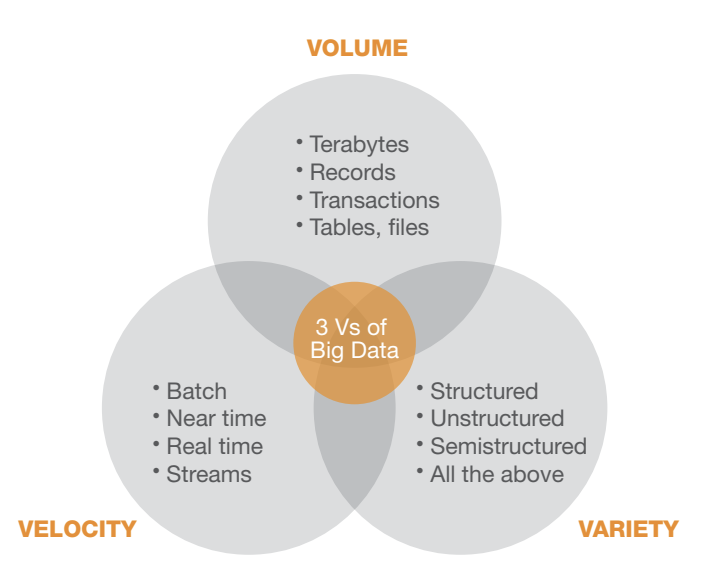
\includegraphics[width=0.5\textwidth]{images/big_data.png}
    \caption{Big Data: 3 V's \autocite{3vbigdata}}
    \label{bigData}
\end{figure}

Beyond these three V's, Big Data is also about how complicated the computing
problem is. Given the number of variables and number of data points for analysing the maritime shipping data. It is a very complicated problem.
Thus, in addition to the three V's identified by IBM, it would also be necessary to take complexity into account as shown in figure \ref*{bigDataComplex} \autocite{pence2014big}.

\begin{figure}[h]
    \centering
    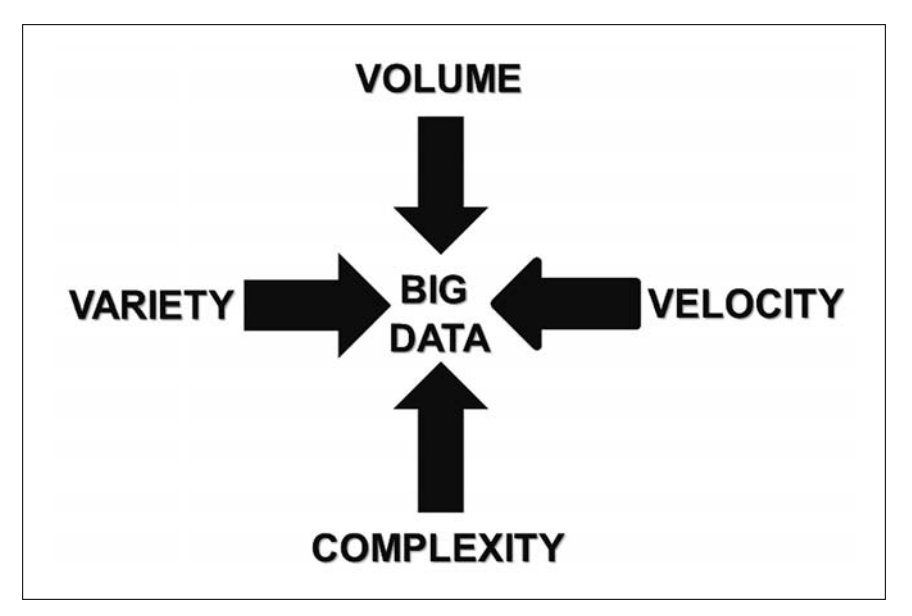
\includegraphics[width=0.5\textwidth]{images/big_data_complex.png}
    \caption{Big Data: Beyong 3 V's - volume, velocity,
        variety, and complexity}
    \label{bigDataComplex}
\end{figure}


\subsection{What is Big Data Analytics?}

Big data analytics is the process of examining large and varied data sets to uncover hidden patterns, unknown correlations, market trends, customer preferences and other useful information that can help organizations make more-informed business decisions.

Thus, Data analytics revolves around deriving valuable knowledge and meaningful insights from extensive sets of data.
This process involves crafting hypotheses, often rooted in gathered experiences and uncovering correlations between variables, sometimes even through serendipitous discoveries.
Data analytics can be classified into four distinct types \autocite{rajaraman2016big}:

\subsubsection{1. Descriptive Analytics}

Descriptive analytics focuses on explaining past events and presenting them in a comprehensible manner.
The collected data is structured into visual aids like bar charts, graphs, pie charts, maps, and scatter diagrams, facilitating easy interpretation that offers insights into the data's implications.
This mode of data representation is often termed a dashboard, reminiscent of a car's dashboard that provides details such as speed, engine status, fuel levels, and distance traveled.
A classic instance of descriptive analytics involves displaying population census data, which categorizes a nation's population by gender, age brackets, education, income, population density, and similar criteria \autocite{rajaraman2016big}.

\subsubsection{2. Predictive Analytics}

Predictive analytics extends beyond existing data to forecast forthcoming events.
It anticipates what is likely to occur in the immediate future.
Techniques like time series analysis utilizing statistical methods, neural networks, and machine learning algorithms are employed for this extrapolation.
A significant application of predictive analytics is seen in marketing, where it understands customer preferences and needs.
For instance, when purchasing shoes online, an advertisement for socks may appear.
Another prevalent application is in orchestrating election campaigns.
This involves gathering diverse data, such as the demographics of voters in different areas and their perceived needs like infrastructure and local concerns \autocite{rajaraman2016big}.

\subsubsection{3. Prescriptive Analytics}

This process detects opportunities for enhancing existing solutions by analyzing collected data.
Essentially, it guides us on the actions to undertake in order to accomplish a particular objective.
An illustrative instance is observed in the aviation industry where airlines determine seat pricing through analysis of historical travel patterns, popular travel origins and destinations, significant events, holidays, and more.
This approach is employed to optimize profit generation \autocite{rajaraman2016big}.

\subsubsection{4. Exploratory or Discovery Analytics}

This process uncovers unforeseen connections among variables within extensive datasets.
The collection and analysis of data from diverse sources opens up new avenues for gaining insights and making serendipitous discoveries.
One of its major applications involves the identification of patterns in customers' behavior by companies through sources like feedback, tweets, blogs, Facebook data, emails, and sales trends.
By deciphering customer behavior, companies can potentially predict actions like renewing a magazine subscription, switching mobile phone service providers, or canceling a hotel reservation. Armed with this information, companies can devise appealing offers aimed at altering the anticipated course of action by the customer \autocite{rajaraman2016big}.
\section{Problem Statement}

Carbon emissions from maritime shipping have been identified as a major contributor to global greenhouse gas emissions, with the International Maritime Organization estimating that shipping is responsible for around 3\% of global CO2 emissions \autocite{king_anthony_2022}.
To address this issue, the shipping industry has set targets to reduce its carbon footprint, and governments and international organizations have introduced policies and regulations to encourage emissions reduction.

However, measuring and monitoring carbon emissions from maritime shipping can be challenging due to the complexity of the industry and the lack of reliable data.
The Energy Efficiency Existing Ship Index (EEXI) and the Carbon Intensity Indicator (CII) have been proposed as two metrics to assess the carbon efficiency of ships and enable comparison between different vessels and fleets \autocite{ZHANG2019118223,CHUAH2023115348}.
However, there is a need to better understand the relationship between EEXI and carbon emissions, as well as to identify the factors that influence EEXI.

Therefore, the aim of this thesis is to conduct a big data analysis of carbon emissions in maritime shipping, using EEXI as the main metric. Specifically, the study will:

\begin{itemize}
    \item Calculate EEXI for a sample of vessels using real-world data on fuel consumption and other operational parameters.
    \item Analyze the relationship between EEOI, CII, and carbon emissions, using statistical methods and machine learning algorithms.
    \item Identify the factors that influence EEXI and CII, such as vessel age, size, speed, and route, and examine their impact on carbon emissions.
    \item Evaluate the usefulness of EEXI and CII as metrics for monitoring and reducing carbon emissions in maritime shipping, and recommend potential improvements to these metrics.
\end{itemize}


Overall, the findings of this thesis will contribute to a better understanding of the carbon efficiency of maritime shipping and inform the development of policies and strategies for emissions reduction in this sector.
\section{Research Question}

This theis will focus on answering following research questions:

\begin{enumerate}
    \item What is the relationship between vessel age and carbon emissions in maritime shipping?
    \item How do shipping routes affect carbon emissions in maritime shipping?
    \item What role do fuel types and engine technologies play in carbon emissions in maritime shipping?
    \item How can EEOI and CII be used to monitor and reduce carbon emissions in maritime shipping?
\end{enumerate}
\section{Report Outline}

\begin{figure}[ht]
    \centering
    \includegraphics[width=1\textwidth]{images/thesis_outline.png}
    \caption{Outline of the thesis}
    \label{fig:outline}
\end{figure}

\noindent Chapter 2: Litrature Review: This chapter covers the background information and literature review of the thesis.
this section covers comprehensive review of existing papers and research related to carbon emissions in maritime shipping.
The aim is to provide a comprehensive overview of the current state of research in this field and identify any gaps or opportunities for further exploration.


\noindent Chapter 3: Data Collection and Understanding:
In this chapter, the focus will be on gathering and understanding the data required to perform analysis to understand emissions in martime shipping.
Various data sources will be explored, including industry databases, research publications, and government reports.
The aim is to acquire a comprehensive dataset that covers different aspects of carbon emissions in the maritime sector.
Additionally, this chapter will delve into the intricacies of the collected data, understanding its structure, variables, and potential limitations.

\noindent Chapter 4: Data Cleaning and Preprocessing:
Before conducting any data analysis, it is crucial to ensure the quality and integrity of the dataset.
This chapter will discuss the steps involved in cleaning and preprocessing the data.
This process may involve handling missing values, dealing with outliers, standardizing formats, and resolving inconsistencies.
By performing these necessary data cleaning procedures, the dataset will be prepared for further analysis, ensuring reliable and accurate results.

\noindent Chapter 5: Data Analysis Techniques:
In this chapter, various data analysis techniques specific to big data will be explored and applied to the cleaned dataset.
These techniques may include statistical analysis, machine learning algorithms, and data visualization methods.
The goal is to extract meaningful insights and patterns from the data to gain a comprehensive understanding of carbon emissions in maritime shipping.
Additionally, this chapter will discuss the tools and technologies utilized for data analysis and highlight any specific challenges encountered during the process.

\noindent Chapter 6: Evaluation of Results:
After performing the data analysis, this chapter will focus on evaluating and interpreting the obtained results.
The findings will be compared against existing literature, industry benchmarks, and regulatory standards to assess the significance and implications of the analysis.
The strengths and limitations of the analysis approach will be discussed, and recommendations for future research or practical applications will be provided.
This chapter aims to provide a comprehensive evaluation of the insights gained from the data analysis and their potential impact on the maritime shipping industry.

\noindent Conclusion:
The conclusion chapter will summarize the key findings and contributions of the thesis.
It will highlight the significance of the conducted big data analysis on emissions in maritime shipping and its implications for sustainability and environmental initiatives.
The conclusion will also discuss any potential limitations or challenges encountered during the research and suggest avenues for further exploration in this field.